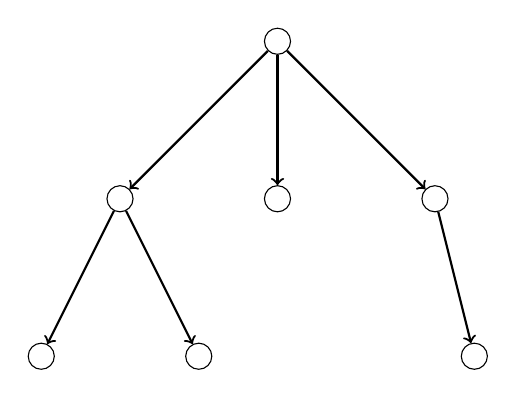
\begin{tikzpicture}
  % Root node
  \node[circle, draw, fill=white] (root) at (0, 0) {};

  % First generation
  \node[circle, draw, fill=white] (g1a) at (-2, -2) {};
  \node[circle, draw, fill=white] (g1b) at (0, -2) {};
  \node[circle, draw, fill=white] (g1c) at (2, -2) {};

  % Second generation from g1a
  \node[circle, draw, fill=white] (g2a) at (-3, -4) {};
  \node[circle, draw, fill=white] (g2b) at (-1, -4) {};

  \node[circle, draw, fill=white] (g2f) at (2.5, -4) {};

  % Edges from root to first generation
  \draw[->, thick] (root) -- (g1a);
  \draw[->, thick] (root) -- (g1b);
  \draw[->, thick] (root) -- (g1c);

  % Edges from g1a to second generation
  \draw[->, thick] (g1a) -- (g2a);
  \draw[->, thick] (g1a) -- (g2b);
  \draw[->, thick] (g1c) -- (g2f);

\end{tikzpicture}